\documentclass{article}
\usepackage[english]{babel}
\usepackage[utf8]{inputenc}
\usepackage{fancyhdr}
\usepackage{geometry}
\usepackage{enumitem}
\usepackage{amsmath}
\usepackage{graphicx}
\usepackage{tcolorbox}
\usepackage{amssymb}
\usepackage[thinc]{esdiff}
\usepackage{float}

\geometry{letterpaper, portrait, margin=1in}
\graphicspath{ {images/} }
\pagestyle{fancy}
\fancyhf{}
\lhead{Keerthik Muruganandam}
\rhead{Yadavalli Homework 1}

\begin{document}

\begin{enumerate}[label=\textbf{(1.\arabic*)}] %%%%%%%%%%%%%%%%%%%%%%%%%%%%%%%%%%%%%%%%%%%%%%%%%%%%%%%%%%%%%%

\item The velocity of a moving particle at time \textit{t} is given by $v(t)=\sin(t)$. %%%
\begin{enumerate}[label=\textbf{(\alph*)}]
\item Find the \textit{net distance} traveled by the particle from $t=0$ to $t=\dfrac{3\pi}{2}$. %%
To find the net distance traveled in the time of 0 to $\dfrac{3\pi}{2}$, simply take the integral of $v(t)$.
\[ \int_a^b\!(v(t))\,\text{d}   =   \int_0^{3\pi/2}\!(\sin(t))\,\text{d}x\]
Next apply the Evaluation Theorem, which states $ \int_{a}^b \! (v(t)) \, \text{d}x=F(b)-F(a)$ when $f(x)$ is continuous on $[a,b]$ and $F$ is any antiderivative of $f$, to the integral.
\[\int_0^{3\pi/2}\!(\sin(t))\,\text{d}x   =   -\cos\left(\frac{3\pi}{2}\right)-\left(-\cos\left(0\right)\right)\]
All that is left is to simplify the expression above to find the integral
\begin{align*}
-\cos\left(\frac{3\pi}{2}\right)-\left(-\cos\left(0\right)\right)&=-\cos\left(\frac{3\pi}{2}\right)+\cos\left(0\right) \\
&= 1
\end{align*}
Now we know the value of $F(b)-F(a)$ is $1$, so
\[\int_0^{3\pi/2}\!(\sin(t))\,\text{d}x = 1\]

\item Find the \textit{total distance} traveled by the particle from $t=0$ to $t=\dfrac{3\pi}{2}$. %%
Finding the total distance is similar to finding the net distance, but instead take $|f(x)|$ instead of plain $f(x)$. The integral of $v(t)$ is negative from $\pi\le t\le3\pi/2$ so we take the integral of $-\sin(t)$ on that interval to turn the negative area positive.Thus there are two integrals.
\[\int_0^\pi \! \sin(x) \, \text{d}x + \int_\pi^{3\pi/2}\! \left(-\sin(x)\right) \, \text{d}x\]
We know that the antiderivative of $\sin(x)$ is $-\cos(x)$ and inversely $-\sin(x)$'s antiderivative is $\cos(x)$, so we can use the Evaluation Theorem we used before to get the expression below.
\[\left(-\cos\left(\pi\right)-\left(-\cos\left(0\right)\right)\right)+\left(\cos\left(\frac{3\pi}{2}\right)-\cos\left(\pi\right)\right)\]
Which simplifies to
\begin{align*}
-(-1 )-(-(1))+0-(-1)&=1+1+0+1 \\
&= 3
\end{align*}
Thus, 
\[\int_0^\pi \! \sin(x) \, \text{d}x + \int_\pi^{3\pi/2}\! \left(-\sin(x)\right) \, \text{d}x=3\]
Therefore the total distance traveled by the particle from $t=0$ to $t=\dfrac{3\pi}{2}$ is 3.
\end{enumerate}

\newpage %%%%%%%%%%%%%%%%%%%%%%%%%%%%%%%%%%%%%%%%%%%%%%%%%%%%%%%%%%%%%%%%%%%%%%%%%%%%%%%

\item Algebraically evaluate the integral ${\displaystyle \int_{-1}^2\!\left(x^2+|x|\right)\,\text{d}x }$. \\ %%%
\newline
First we split the integrals into two separate integrals.
\[\int_{-1}^2\! x^2 \, \text{d}x+\int_{-1}^2\!\left(|x|\right)\,\text{d}x\]
Then we split the integral of $|x|$ again with two different bounds of $(-1,0)$ and $(0,2)$.
\[\int_{-1}^2\! x^2 \, \text{d}x-\int_{-1}^0\!x\,\text{d}x+\int_0^2\!x\,\text{d}x\]
The second integral is negative because the function of $|x|=-x$ on (-1,0) and we can take the constant $-1$ out of $f(x)$. 
\[|x| = \begin{cases}
-x, \text{ if } x \le 0 \\
x, \text{     if } x > 0
\end{cases} \]
Next we can use the Evaluation Theorem and create a simple expression which we can then substitute into. We need to find the antiderivative of $x$ and $x^2$ first. We know that the antiderivative of $x^n=\dfrac{x^{n+1}}{n+1}$ so the antiderivative of $x$ is $\dfrac{x^2}{2}$ and the antiderivative of $x^2$ is $\dfrac{x^3}{3}$. Thus we compute the expression
\begin{align*}
\left[\frac{x^3}{3}\right]_{-1}^2-\left[\frac{x^2}{2}\right]_{-1}^0+\left[\frac{x^2}{2}\right]_0^2&=\frac{2^3}{3}-\frac{{-1}^3}{3}-\left(\frac{0^2}{2}-\frac{{-1}^2}{2}\right)+\frac{2^2}{2}-\frac{0^2}{2} \\
&=\frac{8}{3}+\frac{1}{3}+\frac{1}{2}+\frac{4}{2} \\
&=\frac{9}{3}+\frac{5}{2} \\
&=5+\frac{1}{2} \\
&=\frac{11}{2}
\end{align*}
Now that we know what the value of the sum of our three integrals is, we can loop it back to the original problem and say that
\[\int_{-1}^2\!\left(x^2+|x|\right)\,\text{d}x=\frac{11}{2}\]

\newpage %%%%%%%%%%%%%%%%%%%%%%%%%%%%%%%%%%%%%%%%%%%%%%%%%%%%%%%%%%%%%%%%%%%%%%%%%%%%%%%

\item Find the area of the shaded region below. %%%
\begin{figure}[H]
  \centering
  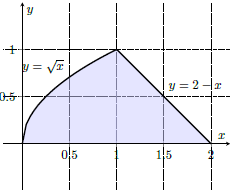
\includegraphics{twoIntegral}
\end{figure}
\begin{enumerate}[label=\textbf{(\alph*)}]

\item by evaluating two integrals with respect to $x$, %%
We can see from the graph that the integral of $\sqrt{x}$ is what is used from (0,1) and the integral of $2-x$ has been used from (1,2). Thus we get the integrals
\[\int_0^1\!\sqrt{x}\,\text{d}x+\int_1^2\!(2-x)\,\text{d}x\]
Next we find the antiderivatives of $\sqrt{x}$ and $2-x$. The former is equal to $x^{1/2}$ so the antiderivative is $\frac{2 {x}^{3/2}}{3}$ and the anti derivative of $2-x$ is $2x-\frac{x^2}{2}$. Next we use the Evaluation Theorem to solve.
\begin{align*}
\frac{2\cdot1^{3/2}}{3}+\left(2\cdot2-\frac{2^2}{2}\right)-\left(2\cdot1-\frac{1^2}{2}\right)&=\frac{2}{3}+4-2-2+\frac{1}{2}\\&=\frac{2}{3}+\frac{1}{2}\\&=\frac{7}{6}
\end{align*}
The area of the shaded region is 7/6.

\item by evaluating one integral with respect to $y$. %%
To do this, first we must get our functions in terms of $y$. $2-x=y$ becomes $2-y=x$ and $y=\sqrt{x}$ becomes $x=y^2$. New we look back at our graph to see that we can take the integral of $2-y$ on (0,1) and then subtract the unshaded area, which is conveniently equal to the integral of $y^2$ on (0,1). Thus we have the set up for our original integral expression
\[ \int_0^1 \! (2-y)\,\text{d}y-\int_0^1\!y^2\,\text{d}y\]
Since both are on the same interval, unlike when we calculated with respect to $x$ we can combine their functions to get
\[\int\!(2-y-y^2)\,\text{d}x\]
Now we can solve using the Evaluation Theorem as usual. But first we need to find the antiderivative which we can find easily using the property $\int\!x^n\,\text{d}x=\frac{x^{n+1}}{n+1}+\text{C}$. Thus the antiderivative is
\[2y-\frac{y^2}{2}-\frac{y^3}{3}\]
Now we can solve.
\[\left(2\cdot1-\frac{1^2}{2}-\frac{1^3}{3}\right)-\left(2\cdot0-\frac{0^2}{2}-\frac{0^3}{3}\right)=2-\frac{1}{2}-\frac{1}{3}=\frac{7}{6}\]
Checking above, both of our answers match and we have found the shaded area with both one and two integrals.
\end{enumerate}

\newpage %%%%%%%%%%%%%%%%%%%%%%%%%%%%%%%%%%%%%%%%%%%%%%%%%%%%%%%%%%%%%%%%%%%%%%%%%%%%%%%

\item \textbf{Professional Problem} Let $F(x)={\displaystyle \int_2^x\!f(t)\,\text{d}t }$. the graph of $f$ is given below. Determine the largest and smallest values of $F(0)$, $F(2)$, $F(3)$, $F(4)$, $F(5)$. \\
\begin{figure}[H]
\centering
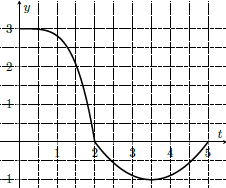
\includegraphics{firstprof}
\end{figure}

Let's start by analyzing the graph and what it means for our integrals. First of all, we observe that all of the integrals are negative \textit{except} $F(2)$. This is because $F(3)$, $F(4)$, $F(5)$ have the entire graph below $y=0$ so the integral is negative. For $F(0)$, the integral in $F(x)$ will be from (2,0). Since $a>b$ in the integral ${\displaystyle \int_a^b\!f(t)\,\text{d}t }$, the function of 0 will also be negative. This is because when calculating $\Delta x$ in the limit definition of the definite integral, $\dfrac{b-a}{n}=-\left(\frac{a-b}{n}\right)$. From this we can conclude that $F(2)$ is the greatest because $0>x$ for all negative $x$.\\
\newline
Now to find the smallest value out of $F(0)$, $F(3)$, $F(4)$, $F(5)$ we will look back at the graph. If we take into account the y-values on the y-axis we see that $f(3)$, $f(4)$, and $f(5)$ are all less than 5. Now if we use the distance 3, 4, 5 are from 2, we notice that their integrals cannot be less than $-$1, $-$2, $-$3. On the other hand, if we try to take $F(0)$ we see that at the minimum it is less than $-$3. How we came to this conclusion is that if we take the line $g(x)=\dfrac{-3}{2}x+3$ it cuts directly across $F(0)$. Since $g(x)$ is lower than $f(x)$ at all points on (0,2), $F(x)$ must be less than the integral of $g(x)$ on (2,0)
\[\int_2^0 \left(-\frac{3}{2}x+3\right)\,\text{d}x=-3\]
Now we have proved that $F(0)$ is less than -3 we know that $F(0)$ must be the least out the given choices because it is least than $-3$ which is the absolute least that $F(5)$ was able to go. Along with the fact $F(5)$ was the had the smallest output out of $F(3)$, $F(4)$, and $F(5)$, we can confidently say that $F(0)$ and $F(2)$ have the smallest and greatest values respectively out of  $F(0)$, $F(2)$, $F(3)$, $F(4)$, $F(5)$.

\end{enumerate}%%%%%%%%%%%%%%%%%%%%%%%%%%%%%%%%%%%%%%%%%%%%%%%%%%%%%%%%%%%%%%%%%%%%%%%%%%%%


\end{document}